\chapter{ActivityNet系统设计}

\section{SAE概述}
考虑到系统将来的可扩展性,我们选择SAE作为系统底层架构。SAE全称为Social Analytic Engine,即社交网络分析引擎,是清华大学计算机系KEG研究组开发的一套社交网络分析平台。可以提供以下功能:
\begin{enumerate}
\item 存储和快速检索极大规模社交网络的数据
\item 提供最新的社交网络分析算法和机器学习算法,如话题模型(Topic Model), 影响力最大化(Influence Maximization)等
\item 提供通用的网络分析引擎和机器学习引擎,
\end{enumerate}

\begin{figure}[!h]
\centering
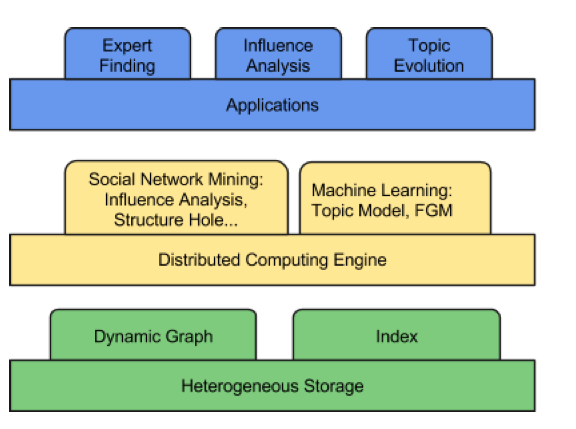
\includegraphics[width=0.7\textwidth]{sae.png}
\caption{SAE基本结构}
\label{fig:sae_arch}
\end{figure}

\section{底层存储}

\section{界面和功能设计}
